\documentclass{beamer}
\usetheme{Warsaw}
\useinnertheme{circles}
\useoutertheme[subsection=false]{smoothbars}
\usepackage[utf8x]{inputenc}
\usepackage[czech]{babel}
\usepackage[T1]{fontenc}
\usepackage{listings}
\usepackage{tikz}

\begin{document}

\AtBeginSection[]
{
  \begin{frame}
    \frametitle{Outline}
    \tableofcontents[currentsection]
  \end{frame}
}

\title{Open source programování}
\subtitle{Open source projekty}
\author{Petr Baudiš $\langle${\tt pasky@ucw.cz}$\rangle$}
\institute{MFF UK 2012\\
	\vskip 1ex
	\pgfdeclareimage[height=4ex]{ccbysa}{by-sa.pdf}
	\pgfuseimage{ccbysa}
}
\date{}
\frame{\titlepage}

\section{Úvod}

\subsection{}
\begin{frame}{O čem dnes}
\begin{center}
{\bf Otevřené projekty II}
\end{center}
\begin{itemize}
\item Osobní zkušenosti: ELinks, GNU libc, Pachi
\item Linuxové distribuce! Debian, openSUSE, \dots
\item \dots ale také Wikipedia nebo RepRap.
\end{itemize}
\end{frame}


\section{Osobní zkušenosti}

\subsection{}
\begin{frame}{ELinks}
\begin{itemize}
\item Fork Linksu od roku 2001 (links-pb $\to$ links-hacked $\to$ Experimental Links $\to$ Enhanced Links), Petr Baudiš $\to$ Jonas Fonseca $\to$ Kalle Olavi Niemitalo, GPL
\item Projekt ve spánku a bez jasného maintainera (zralý na fork?); neaktivní mailing list, bugzilla, git
\item Vývoj stylem benevolent dictator nefunguje bez diktátora
\item Nesmyslný release schedule --- realistické a {\em volné} cíle
\item Perfect is enemy of good
\end{itemize}
\end{frame}

\subsection{}
\begin{frame}{glibc}
\begin{itemize}
\item Jeden z hlavních GNU projektů
\item GPLv2 (!), copyright assignment required
\item Obrovský moloch, obskurní kód a technologie
\item Problém jménem Ulrich Drepper (\dots exkurze v bugzille)
\item Řešení: (0) steering committee (i) formální procesy \\ (ii) Goldman Sachs
\end{itemize}
\end{frame}

\subsection{}
\begin{frame}{Pachi}
\begin{itemize}
\item Od roku 2007, projekt 1-2 lidí (Petr Baudiš, Jean-loup Gailly), GPL (původně část MIT)
\item Vývoj: konflikt mezi open source a snahou o prvenství ve vědeckých výsledcích a turnajích
\item Málo dobrovolníků :-( a pochybně responsivní maintainer
\item Release schedule: ``když se nám chce'' :-)
\end{itemize}
\end{frame}


\section{Distribuce}

\subsection{}
\begin{frame}{Debian}
\begin{itemize}
\item Bugreporty pres Debian BTS
\item Začátek: Non-maintainer uploads (NMU), sponsoři
\item Časem se člověk stane maintainerem; archivy spravují uploadeři
\item Technické otázky: konsensus
\item Debian Project:
	\begin{itemize}
	\item Debian Social Contract, DFSG, Debian Constitution
	\item Project Leader, Secretary, Technical Committee
	\item Demokratická organizace projektu (jako Apache)
	\end{itemize}
\end{itemize}
\end{frame}

\subsection{}
\begin{frame}{OpenSUSE}
\begin{itemize}
\item Zázemí Novell / SUSE, snaha předat vývoj komunitě se moc nedaří
\item OpenSUSE Build Service
\item \dots Stickova prezentace \dots
\end{itemize}
\end{frame}


\section{Netradiční projekty}

\subsection{}
\begin{frame}{Wikipedia}
\begin{itemize}
\item Wikipedia není demokracie, vláda ``hrubého konsensu''
\item Pravidla editována společně, problémy primárně řešeny diskusí
\item Častý výskyt ``ideologických'' sporů
\vskip 4ex
\item {\em Technické} role: Správci, sysopové, byrokrati \dots \\
		accountability, předcházení revert válkám
\item {\em Technicko-politické} role: Stevardi (Wikimedia foundation)
\item {\em Politické} role (prakticky neomezené pravomoc): Arbitrážní komise, Jimmy Wales
\end{itemize}
\end{frame}

\subsection{}
\begin{frame}{RepRap}
\begin{itemize}
\item RepRap is humanity's first general-\\purpose self-replicating manufacturing \\ machine.
\item 3D tiskárna z plastu, důraz na co \\ nejjednodušší a nejvytisknutelnější \\ konstrukci.
\item Ideologický cíl vs. praktické problémy; \\ rostou alternativy jako MakerBot nebo \\ Easy3DMaker.
\item Zdrojáky: SCAD soubory; GPLv2 {\footnotesize (For this purpose the words "software" and "library" in the GNU General Public Licence are taken to mean any and all computer programs computer files designs images videos sound recordings data results documents and all other copyright information available from the RepRap project.)}
\item Vývoj: Málo explicitních releasů. GitHub a pull requesty! https://github.com/prusajr/PrusaMendel
\end{itemize}
\begin{tikzpicture}[remember picture,overlay]
  \node [xshift=-4.75cm,yshift=-6cm,above right] at (current page.north east)
      {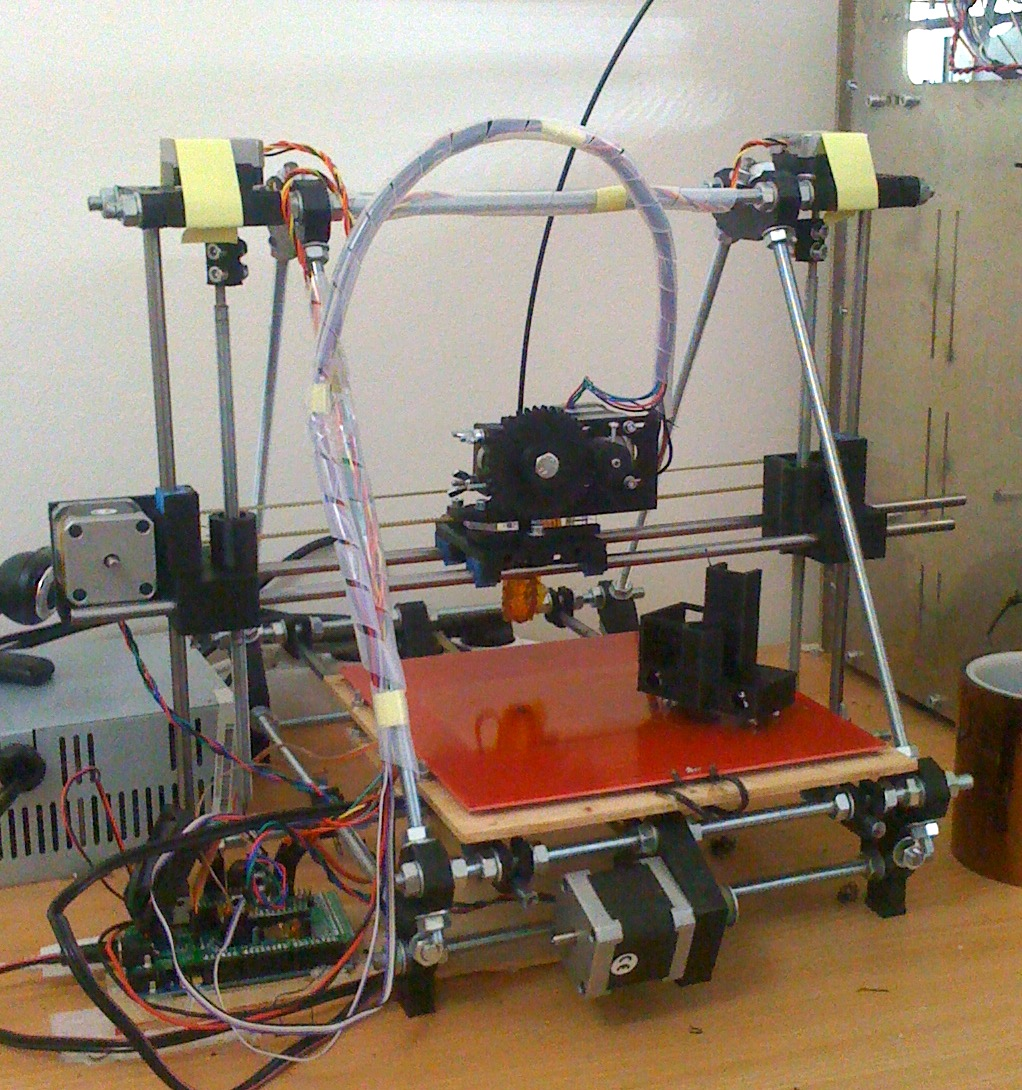
\includegraphics[width=4cm]{Assembled-prusa-mendel.jpg}};
\end{tikzpicture}
\end{frame}


\subsection{}
\begin{frame}{Děkuji za pozornost}
\begin{center}
Příště: Architektura Linuxu a vývojové prostředí.
\end{center}
\end{frame}

\end{document}
